% Options for packages loaded elsewhere
\PassOptionsToPackage{unicode}{hyperref}
\PassOptionsToPackage{hyphens}{url}
\PassOptionsToPackage{dvipsnames,svgnames,x11names}{xcolor}
%
\documentclass[
  letterpaper,
  DIV=11,
  numbers=noendperiod]{scrartcl}

\usepackage{amsmath,amssymb}
\usepackage{iftex}
\ifPDFTeX
  \usepackage[T1]{fontenc}
  \usepackage[utf8]{inputenc}
  \usepackage{textcomp} % provide euro and other symbols
\else % if luatex or xetex
  \usepackage{unicode-math}
  \defaultfontfeatures{Scale=MatchLowercase}
  \defaultfontfeatures[\rmfamily]{Ligatures=TeX,Scale=1}
\fi
\usepackage{lmodern}
\ifPDFTeX\else  
    % xetex/luatex font selection
\fi
% Use upquote if available, for straight quotes in verbatim environments
\IfFileExists{upquote.sty}{\usepackage{upquote}}{}
\IfFileExists{microtype.sty}{% use microtype if available
  \usepackage[]{microtype}
  \UseMicrotypeSet[protrusion]{basicmath} % disable protrusion for tt fonts
}{}
\makeatletter
\@ifundefined{KOMAClassName}{% if non-KOMA class
  \IfFileExists{parskip.sty}{%
    \usepackage{parskip}
  }{% else
    \setlength{\parindent}{0pt}
    \setlength{\parskip}{6pt plus 2pt minus 1pt}}
}{% if KOMA class
  \KOMAoptions{parskip=half}}
\makeatother
\usepackage{xcolor}
\setlength{\emergencystretch}{3em} % prevent overfull lines
\setcounter{secnumdepth}{-\maxdimen} % remove section numbering
% Make \paragraph and \subparagraph free-standing
\ifx\paragraph\undefined\else
  \let\oldparagraph\paragraph
  \renewcommand{\paragraph}[1]{\oldparagraph{#1}\mbox{}}
\fi
\ifx\subparagraph\undefined\else
  \let\oldsubparagraph\subparagraph
  \renewcommand{\subparagraph}[1]{\oldsubparagraph{#1}\mbox{}}
\fi


\providecommand{\tightlist}{%
  \setlength{\itemsep}{0pt}\setlength{\parskip}{0pt}}\usepackage{longtable,booktabs,array}
\usepackage{calc} % for calculating minipage widths
% Correct order of tables after \paragraph or \subparagraph
\usepackage{etoolbox}
\makeatletter
\patchcmd\longtable{\par}{\if@noskipsec\mbox{}\fi\par}{}{}
\makeatother
% Allow footnotes in longtable head/foot
\IfFileExists{footnotehyper.sty}{\usepackage{footnotehyper}}{\usepackage{footnote}}
\makesavenoteenv{longtable}
\usepackage{graphicx}
\makeatletter
\def\maxwidth{\ifdim\Gin@nat@width>\linewidth\linewidth\else\Gin@nat@width\fi}
\def\maxheight{\ifdim\Gin@nat@height>\textheight\textheight\else\Gin@nat@height\fi}
\makeatother
% Scale images if necessary, so that they will not overflow the page
% margins by default, and it is still possible to overwrite the defaults
% using explicit options in \includegraphics[width, height, ...]{}
\setkeys{Gin}{width=\maxwidth,height=\maxheight,keepaspectratio}
% Set default figure placement to htbp
\makeatletter
\def\fps@figure{htbp}
\makeatother
\newlength{\cslhangindent}
\setlength{\cslhangindent}{1.5em}
\newlength{\csllabelwidth}
\setlength{\csllabelwidth}{3em}
\newlength{\cslentryspacingunit} % times entry-spacing
\setlength{\cslentryspacingunit}{\parskip}
\newenvironment{CSLReferences}[2] % #1 hanging-ident, #2 entry spacing
 {% don't indent paragraphs
  \setlength{\parindent}{0pt}
  % turn on hanging indent if param 1 is 1
  \ifodd #1
  \let\oldpar\par
  \def\par{\hangindent=\cslhangindent\oldpar}
  \fi
  % set entry spacing
  \setlength{\parskip}{#2\cslentryspacingunit}
 }%
 {}
\usepackage{calc}
\newcommand{\CSLBlock}[1]{#1\hfill\break}
\newcommand{\CSLLeftMargin}[1]{\parbox[t]{\csllabelwidth}{#1}}
\newcommand{\CSLRightInline}[1]{\parbox[t]{\linewidth - \csllabelwidth}{#1}\break}
\newcommand{\CSLIndent}[1]{\hspace{\cslhangindent}#1}

\usepackage{booktabs}
\usepackage{caption}
\usepackage{longtable}
\usepackage{colortbl}
\usepackage{array}
\KOMAoption{captions}{tableheading}
\makeatletter
\makeatother
\makeatletter
\makeatother
\makeatletter
\@ifpackageloaded{caption}{}{\usepackage{caption}}
\AtBeginDocument{%
\ifdefined\contentsname
  \renewcommand*\contentsname{Table of contents}
\else
  \newcommand\contentsname{Table of contents}
\fi
\ifdefined\listfigurename
  \renewcommand*\listfigurename{List of Figures}
\else
  \newcommand\listfigurename{List of Figures}
\fi
\ifdefined\listtablename
  \renewcommand*\listtablename{List of Tables}
\else
  \newcommand\listtablename{List of Tables}
\fi
\ifdefined\figurename
  \renewcommand*\figurename{Figure}
\else
  \newcommand\figurename{Figure}
\fi
\ifdefined\tablename
  \renewcommand*\tablename{Table}
\else
  \newcommand\tablename{Table}
\fi
}
\@ifpackageloaded{float}{}{\usepackage{float}}
\floatstyle{ruled}
\@ifundefined{c@chapter}{\newfloat{codelisting}{h}{lop}}{\newfloat{codelisting}{h}{lop}[chapter]}
\floatname{codelisting}{Listing}
\newcommand*\listoflistings{\listof{codelisting}{List of Listings}}
\makeatother
\makeatletter
\@ifpackageloaded{caption}{}{\usepackage{caption}}
\@ifpackageloaded{subcaption}{}{\usepackage{subcaption}}
\makeatother
\makeatletter
\@ifpackageloaded{tcolorbox}{}{\usepackage[skins,breakable]{tcolorbox}}
\makeatother
\makeatletter
\@ifundefined{shadecolor}{\definecolor{shadecolor}{rgb}{.97, .97, .97}}
\makeatother
\makeatletter
\makeatother
\makeatletter
\makeatother
\ifLuaTeX
  \usepackage{selnolig}  % disable illegal ligatures
\fi
\IfFileExists{bookmark.sty}{\usepackage{bookmark}}{\usepackage{hyperref}}
\IfFileExists{xurl.sty}{\usepackage{xurl}}{} % add URL line breaks if available
\urlstyle{same} % disable monospaced font for URLs
\hypersetup{
  pdftitle={The Long-Term Impact of Experiencing War on Life Satisfaction - Evidence from the Life in Transition Survey},
  pdfauthor={Jemesa Landers; Tom Coupé; Andrea Menclova},
  pdfkeywords={War, Life
Satisfaction, Replications, Metaverse, Specification Curve},
  colorlinks=true,
  linkcolor={blue},
  filecolor={Maroon},
  citecolor={Blue},
  urlcolor={Blue},
  pdfcreator={LaTeX via pandoc}}

\title{The Long-Term Impact of Experiencing War on Life Satisfaction -
Evidence from the Life in Transition Survey}
\author{Jemesa Landers \and Tom Coupé \and Andrea Menclova}
\date{2024-04-02}

\begin{document}
\maketitle
\begin{abstract}
This paper replicates, evaluates and updates the papers that estimate
the long run impact of experiencing war on life satisfaction using the
Life in Transition Survey. We show that while the published results can
be replicated, conclusions are very sensitive to specification choices
the authors made. Overall, we find little evidence supporting a causal
long-term effect of war experience on life satisfaction.
\end{abstract}
\ifdefined\Shaded\renewenvironment{Shaded}{\begin{tcolorbox}[boxrule=0pt, interior hidden, borderline west={3pt}{0pt}{shadecolor}, enhanced, sharp corners, breakable, frame hidden]}{\end{tcolorbox}}\fi

\hypertarget{i.-introduction.}{%
\subsection{I. Introduction.}\label{i.-introduction.}}

There is a growing literature on the impact of experiencing war on life
satisfaction ( see Coupé and Obrizan (2023) for a recent review).
Interestingly, however, several papers in this literature come to
opposite conclusions even though they use the same dataset, and the same
variables to measure life satisfaction and war.

Using the 2010 wave of the Life in Transition Survey (LITSII), which
covers over 30000 respondents from thirty five European and Central
Asian countries, Kijewski (2020) finds that respondents who were
physically injured, or had parents or grandparents physically injured or
killed during World War II, have significantly lower levels of life
satisfaction, measured on a scale between 1 and 10 (Table 4, −0.108,
p\textless0.01, n=25618). In the paper's abstract, Kijewski (2020)
writes: ``Our findings indicate that war experiences continue to be
related to lower levels of life satisfaction even six decades after the
end of the war''.

However, Ivlevs (2015), also using LITSII, the same war variable and the
same life satisfaction variable (but restricting the sample to those
less than 65 years old), finds a positive and significant effect (Table
2, 0.071, p\textless0.05, n=24070). Ivlevs (2015) explains this positive
effect by referring to the happiness of having survived, to war
increasing ``feelings of shared purpose, solidarity, trust, friendship
and national pride'', and to pride of having ``someone in their family
died as a `martyr' or was fighting for a `good' or `holy' cause'''
(p.~349).

Finally, Child and Nikolova (2020) restricts the LITSII sample to ``15
countries which experienced significant disruption from World War II
battle activity'' and finds no significant effect of the same war
variable on the same life satisfaction variable (Table 8, --0.006,
p\textgreater0.1, n=9538).

Noteably, both Kijewski (2020) and Child and Nikolova (2020) (but not
Ivlevs (2015)) include a second war-related variable, a dummy for
whether the respondent, or any of his/her parents or grandparents were
displaced during World War II, as a control variable. Both estimated
this variable to have a positive and significant effect on life
satisfaction (Table 4, 0.118, p\textless0.01, n=25618, and Table 8,
0.078, p\textless0.01, n=9538, respectively).

Besides these 3 studies, there are two other studies that use the same
LITSII dataset but use slightly different measures of life satisfaction
and/or war experience. Nikolova and Sanfey (2016) convert the 1 to 10
life satisfaction scale into a 1 to 5 scale, and merge both aspects
(being displaced and/or injured/killed in the war) into one war
experience variable, and find no significant effect (Table A1, 0.0241,
p\textgreater0.1, n=25666). In addition, they use a second life
satisfaction question included in LITS II, which is also on a 1 to 5
scale, and again find no significant effect (Table A1, 0.00630,
p\textgreater0.1, n=25427). Using the latter question and the aggregated
war variable, Djankov, Nikolova, and Zilinsky (2016) also find no effect
(Table 5, −0.008, p\textgreater0.1, n=24836).

Table I gives an overview of the characteristics and findings of the
five studies that use LITSII to estimate the relationship between World
War II exposure and life satisfaction.

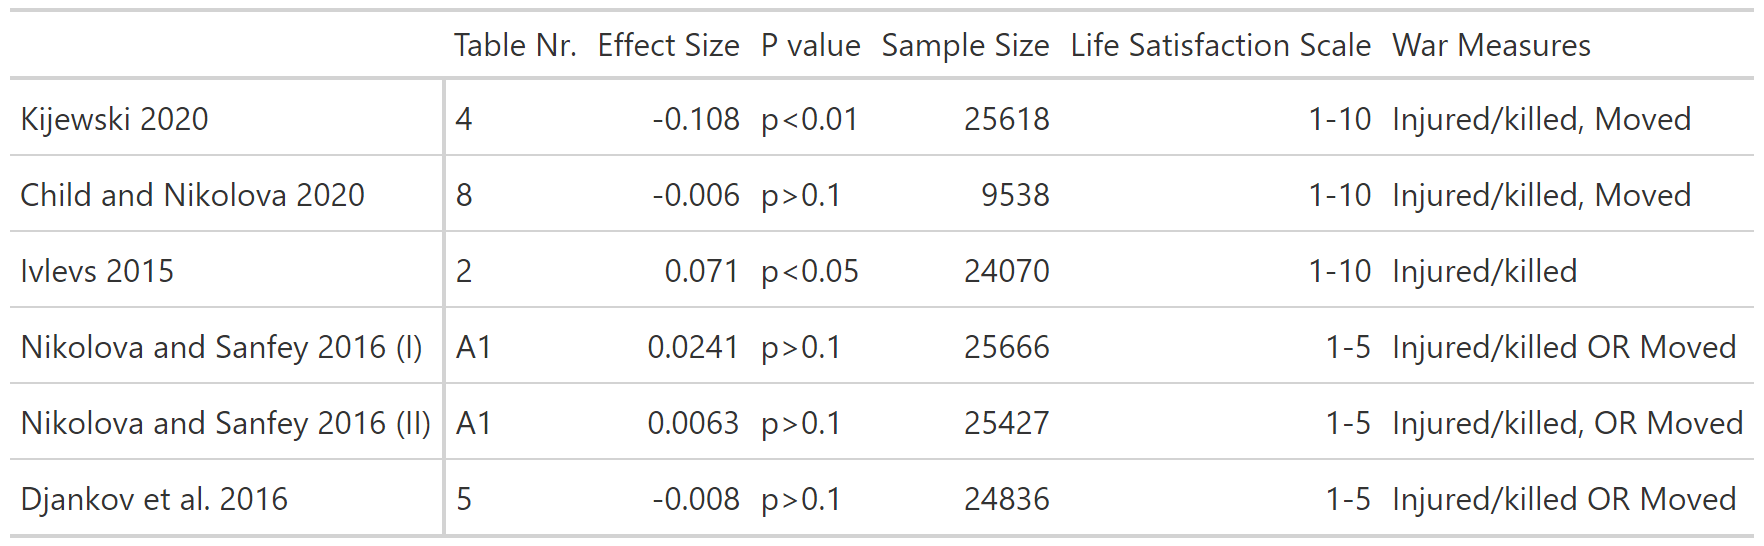
\includegraphics{tab_1.png}

Note that, while the above studies focus on how World War II affects
happiness, none of them allowed for other, more recent and local wars,
to affect happiness, even though questions about victimization and
displacement related to these other wars are available in the LITSII
survey. Moreover, Obrizan (2019), using the third wave of the Life in
Transition Survey (LITSIII), regresses life satisfaction (a happy/not
happy dummy) on these recent war experiences, and finds insignificant
negative effects of having injured or killed household members, but
significant negative effects of having been displaced by these more
recent and local wars (Table 2, -0.063, p\textless0.01, n=18157).
Interestingly, Obrizan (2019) does not allow for World War II experience
to influence life satisfaction.\footnote{Using LITSIII, Adsera et al.
  (2020) measures war experience by whether the respondent was less than
  2 years old during World War II or a more recent war. They do not show
  the estimates of this variable suggesting it was insignificant. Recher
  (2022) regresses the absolute value of the difference between the life
  satisfaction in various locations on differences in war experience
  (both recent wars and World War II), and finds a significant
  relationship. However, given absolute values are taken, one can not
  distinguish whether war has a negative or a positive effect. We will
  not consider these papers as our focus is on the impact of personally
  experiencing the impact of war (rather than living in/being born in a
  country affected by war). Similarly, our analysis ignores the impact
  on the life satisfaction of those killed during the war.}

In this paper, we analyse possible reasons for the conflicting findings
of these previosu studies. We start by replicating the results of table
I. There is ample evidence of a replication crisis in the social
sciences (see for example, Baker (2016) or Reed (2018)), with
researchers being unable to reproduce the results of published papers
when trying to repeat the analysis described in those papers.
Replicating the five papers from Table I will allow us to eliminate the
possibility that the opposing findings are due to coding errors or typos
in the published papers.

We then do perform specification curve analysis. The studies from Table
I taken together make a `real-life' `many analysts project'. In a `many
analysts project' (see, for example, Huntington-Klein et al. (2021), or
in the context of life satisfaction, Hoogeveen et al. (2021)), a
researcher provides a large number of analysts with the same dataset and
research question, and then investigates how their conclusions differ.
Typically, such projects document substantial differences in
methodological choices and in some cases, substantial differences in
conclusions. To show the range of possible outcomes (and avoid
conflicting papers to be published), Simonsohn, Joseph, and Nelson
(2021) propose specification curve analysis, which consists of
conducting joint inference across all `theoretically relevant' and
`statistically valid' specifications. In this paper, we use the
specifications proposed by the five papers as the starting point of a
specification curve analysis, allowing us to assess the degree of model
uncertainty; that is, to what extent different specification choices
lead to different estimates and conclusions.

Finally, we will analyse to what extent the conclusions of the studies
of Table I are stable over time, by using the most recent, third, wave
of the Life in Transition Survey and re-estimating the specifications of
the five original studies. Together, the replication, the specification
curve analysis and the updated analysis will allow us to assess how
strong the evidence, that the Life in Transition Survey can provide, is
about the long-term impact of war on life satisfaction.

Admittedly, it is difficult to obtain causal evidence based on
non-experimental survey data like LITS, as the `treatment' variable is
not randomized. At the same time, it is hard to see how one could
ethically run an experiment to measure the long-term effect of
experiencing war on life satisfaction. While this means the `strongest
support for the causation hypothesis' is out of reach, we can analyse
how well the research on the impact of war on life satisfaction scores
on some of the other Bradford-Hill criteria (Bradford-Hill (1965)) such
as consistency - that is, has the effect `been repeatedly observed by
different persons, in different places, circumstances and times?' - or
the `strength of the association'. Note that within the constraints of
using non-experimental data, LITS has several important advantages. The
survey is large, with tens of thousands of respondents, and has been
implemented in both 2010 (LITSII) and 2016 (LITSIII). It allows to
measure life satisfaction in different ways based on two separate survey
questions. Finally, while few large-scale surveys ask about war
experiences, LITS has five questions related to war experience. Hence,
LITS is one of the best available sources to estimate the long-term
impact of war on life satisfaction.

The remainder of the paper is structured as follows. Section II
replicates the five papers that provide estimates of the impact of World
War II on life satisfaction. Section III provides a specification curve
analysis focusing on the impact of having been physically injured, or
having parents or grandparents who were physically injured or killed
during World War II. Section IV focuses on the impact of having been
displaced during World War II and of having been affected by more recent
wars. Section V analyses the same questions but uses data from the third
wave of LITS, while Section VI concludes.

\hypertarget{ii.-replicating-the-literature.}{%
\subsection{II. Replicating the
literature.}\label{ii.-replicating-the-literature.}}

Given the evidence of a replication crisis in the social sciences (Baker
(2016), Reed (2018)), we want to make sure the conflicting findings
reported by various papers are not the results of typos in the published
versions or errors in the computer codes used to generate these
findings. We therefor replicate the key regressions of these papers by
following the descriptions of the method, included variables and
construction of the variables, provided in the papers.

Table II shows, for each study, the published effect size of the impact
of experiencing injury/death during World War II, the p-value and sample
size (columns I to III), followed by the effect size, p-value and sample
size we get when we replicate these papers' key regressions.

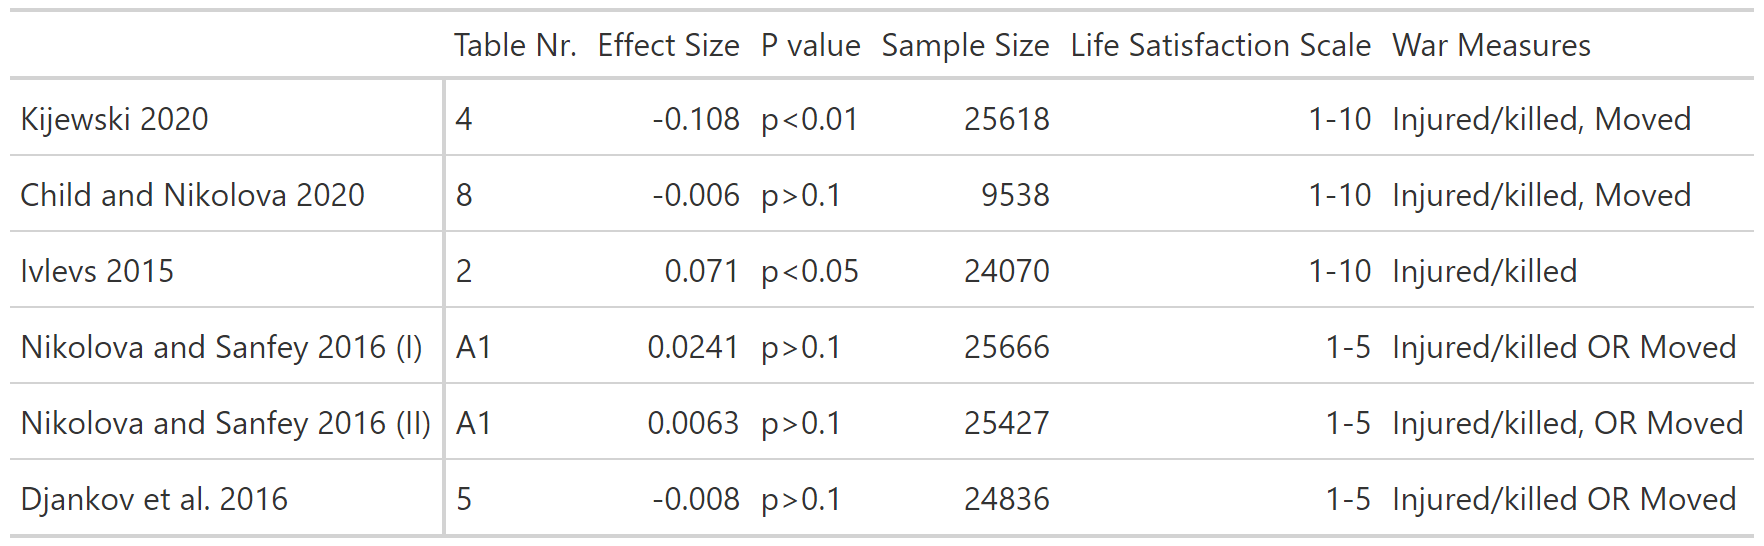
\includegraphics{tab_1.png}

Table II shows that the replicated results for Kijewski (2020), Nikolova
and Sanfey (2016) and Djankov, Nikolova, and Zilinsky (2016) are almost
identical to the published results. There are a couple of minor
exceptions: like Child and Nikolova (2020), we find an insignificant
effect, but the replicated effect size is considerably more negative.
Like Ivlevs (2015), we find a positive estimate. However, unlike Ivlevs
(2015), who found statistical significance at the 5\% level, we only
find the estimated effect to be significant at the 11\% significance
level.

Overall, we successfully replicate the literature estimating the impact
of experiencing World War II on life satisfaction, finding a negative
estimate when the original authors find a negative estimate and a
positive estimate when the original authors find a positive estimate. In
terms of statistical significance, we also come to the same conclusion
as the original authors, except for Ivlevs (2015) for which we find
slightly weaker evidence that the effect is significantly positive.

\hypertarget{iii.-a-specification-curve-analysis.}{%
\subsection{III. A Specification Curve
Analysis.}\label{iii.-a-specification-curve-analysis.}}

To further explore the reasons why different authors find different
estimates, we conduct a specification curve or multiverse analysis
(Simonsohn, Joseph, and Nelson (2021), Steegen et al. (2016)).

The papers we replicated all use the same dataset. However, the authors
use this same dataset in many ways\footnote{One reason for the
  difference in methodological choices could be differences in the goal
  of the analysis: Kijewski (2020) and Child and Nikolova (2020) focuse
  on the impact of war on life satisfaction. Ivlevs (2015) uses war as
  an instrumental variable for life satisfaction, while focusing on what
  drives migration decisions. Djankov, Nikolova, and Zilinsky (2016) and
  Nikolova and Sanfey (2016) use war as a control variable in a
  happiness regression, while focusing on the happiness gap between
  transition and non-transition countries, and differences across
  various measures of life satisfaction respectively.}. As explained in
the introduction, there are differences in what measure of life
satisfaction gets selected (1-5 scale versus 1-10 scale\footnote{The
  1-10 scale comes from the question: ``All things considered, how
  satisfied or dissatisfied are you with your life as a whole -these
  days? Please answer on a scale from 1 to 10, where 1 means completely
  dissatisfied and 10 means completely satisfied.'' The 1 to 5 scale
  comes from the question: `All things considered, I am satisfied with
  my life now', with 1 meaning strongly disagree and 5 meaning strongly
  agree.}) and in how the war variable gets included (only the variable
reflecting injuries/death included, the displacement-by-war variable
also included, or both variables aggregated into one single measure of
war experience).

Some of the control variables are common to all studies. All studies
include variables capturing the age, gender, employment status, marital
status, and health status of the respondent. They also include measures
of the education of the respondent and the respondent's father. All but
Kijewski (2020) include income as a control variable. However, there are
small differences in how authors include these variables: for example,
some include dummies for all categories of education while others
aggregate educational attainment into wider categories.

Besides the common set of control variables, there are many
idiosyncratic variable choices. Kijewski (2020) controls for occupation,
and religious and civic involvement. Child and Nikolova (2020) controls
for mother's education, whether the respondent or family members had
been members of the communist party, whether the respondent had ever
moved, and for rural/urban differences. Ivlevs (2015) controls for
minority status, rural/urban/metropolitan status, whether there are
children in the household, the presence of a migration network,
differences in assets and differences in financial satisfaction.

The authors also chose different ways to capture geographic differences.
Some include country fixed effects (Ivlevs (2015), Nikolova and Sanfey
(2016)), others include in-country region-specific fixed effects (Child
and Nikolova (2020)) while yet others include country random effects in
addition to country-level characteristics like unemployment or per
capita GDP (Kijewski (2020)), or just country-level characteristics such
as whether the country was a transition country (Djankov, Nikolova, and
Zilinsky (2016)).

Studies differ on whether they cluster standard errors and in whether or
not they weigh observations. Kijewski (2020) does not cluster standard
errors nor uses survey weights. All others use within country population
weights (which makes the sample representative for each country, but
also gives each country equal weight overall) and cluster standard
errors at the level of country, region, or locality.

Finally, studies differ in which observations they included: Ivlevs
(2015) focuses on those who are less than 65 years old, Kijewski (2020)
excludes Kosovo, while Child and Nikolova (2020) focus on 15 countries
that were heavily affected by World War II.

To illustrate the impact of methodological differences, Simonsohn,
Joseph, and Nelson (2021) suggest to start from the ``set of
theoretically justified, statistically valid, and non-redundant
specifications''. In this study, we use the specifications chosen by the
five papers as the starting point for our set. While not necessarily
exhaustive, given the choices underlying these specifications have all
been deemed acceptable by these authors, the referees who reviewed these
papers and the editors who decided to accept these papers for
publication, the specifications based on these choices all can be
considered `reasonable'.

More specifically, we use the five weights, clustering, and fixed effect
choices of the papers. We vary what dependent variable is used (1-5
scale versus 1-10 scale), and what sub-population is used (15 heavily
affected countries only, only under 65-year-olds, or a combination of
these two). We include the common control variables in all
specifications\footnote{We use the most flexible specification of this
  common set. That is, we do not aggregate categories of categorical
  variables. We do not include a subset that excludes Kosovo because
  Kosovo represents a very small share of the overall sample (about
  3\%).} but vary the set of additional controls: a set of
income-related variables (income, satisfaction with one's financial
situation, a proxy for assets), a set of additional war experiences
(moved during World War II, moved because of recent conflict, injured
during recent conflict, injured/killed household members during recent
conflict), a set of all remaining controls, and any combination of the
aforementioned sets.

Figure I displays the specification curve, showing the 320 estimated
effect sizes (and their confidence intervals) of the dummy variable
measuring whether or not the respondent, or a family member, was injured
or killed during World War II.\footnote{We use the specr R package
  (Masur and Scharkow (2020)) for the specification analysis and the
  Stargazer package for the regression output (Hlavac (2022))} Estimates
are ordered from smallest to biggest, with statistically significant
estimates at the 5\% significance level highlighted in red (if negative)
or blue (if positive). About 71\% of these estimates are negative. A
substantial part of the negative estimates is statistically significant
(36.2\% overall) but none of the positive estimates are statistically
significant.

Overall, the median estimate is -0.04. Focusing on those specifications
that use the 1-10 life satisfaction scale, the median estimate is
-0.045, those using the 1-5 life satisfaction scale -0.029. These are
small effect sizes when compared to the standard deviation of the 1-10
scale (2.13) or the 1-5 scale (1.09). And even the 5\% percentile
estimate (-0.12) and 95\% percentile estimate (0.03) are small.

Figure I: A Specification Curve for the Impact of Being Injured/Having
Injured or Killed Relatives during World War II on Life Satisfaction.

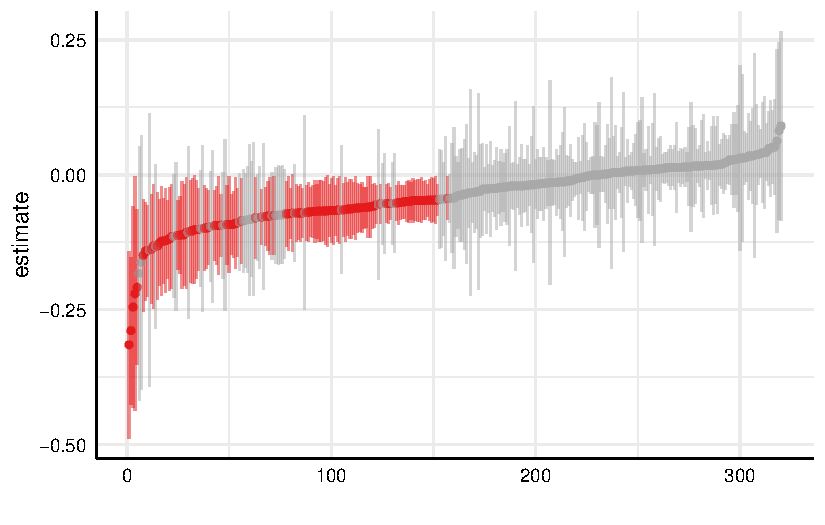
\includegraphics{PAPERLongTermImpactofWaronLifeSatisfaction_files/figure-pdf/results to show Ia-1.pdf}

Figure II shows how estimates differ across models, control variables
included, sample restrictions and dependent variables. The biggest
difference comes from controlling for income. Omitting the income
variables drives the estimated coefficient of the injured/killed war
variable downwards and increases the likelihood the estimate is
statistically significant. In fact, none of the estimated effects are
statistically significant if income variables are included as controls.
This is noteworthy as Kijewski (2020) is the only study that does not
include an income variable as a control and is the only study that finds
a significant negative effect of the injured/killed war variable. There
are good reasons to include income as a control variable as happiness
regressions typically include income, allowing for money to `buy'
happiness. At the same time, one could argue that income is a `bad'
control: if the war variable affects income, controlling for income will
obscure some of the effect of the war on life satisfaction. That being
said, all five papers included health as a control variable, and like
for income one could argue that war experience affects current health
status, and hence, that health should not be included as a control.

Figure II: What Affects the Estimated Effect Size of Being Injured/
Having Injured or Killed relatives during World War II.

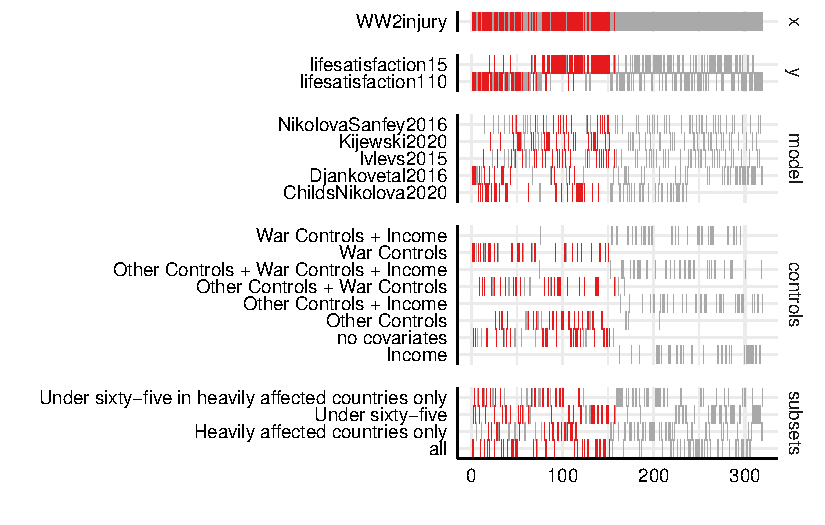
\includegraphics{PAPERLongTermImpactofWaronLifeSatisfaction_files/figure-pdf/results to show Ib-1.pdf}

Other factors matter much less. The regression of estimated effect sizes
on the characteristics of the specifications in Table III shows that,
keeping everything else constant, the model by Child and Nikolova (2020)
has somewhat smaller effect sizes than the models by Djankov, Nikolova,
and Zilinsky (2016), Ivlevs (2015), Kijewski (2020) and Nikolova and
Sanfey (2016). Similarly, using the 1-10 life satisfaction scale results
in somewhat smaller estimates, while differences in who is included in
the sample do not seem to affect the effect sizes much.

\begin{verbatim}

Table III - Correlates of the Estimated Effect Size
=======================================================================================
                                                                Dependent variable:    
                                                            ---------------------------
                                                                   Estimate Size       
---------------------------------------------------------------------------------------
model - Djankovetal2016                                               0.013**          
                                                                      (0.005)          
                                                                                       
model - Ivlevs2015                                                   0.019***          
                                                                      (0.005)          
                                                                                       
model - Kijewski2020                                                 0.020***          
                                                                      (0.005)          
                                                                                       
model - NikolovaSanfey2016                                           0.019***          
                                                                      (0.005)          
                                                                                       
subset- Heavily affected countries only                               -0.002           
                                                                      (0.005)          
                                                                                       
subset- Under sixty-five only                                         0.009*           
                                                                      (0.005)          
                                                                                       
subset- Under sixty-five in heavily affected countries only          -0.011**          
                                                                      (0.005)          
                                                                                       
Controls - No Additional Controls                                    -0.095***         
                                                                      (0.007)          
                                                                                       
Controls - Other Controls                                            -0.077***         
                                                                      (0.007)          
                                                                                       
Controls - Other Controls + Income Controls                            0.001           
                                                                      (0.007)          
                                                                                       
Controls - Other Controls + War Controls                             -0.089***         
                                                                      (0.007)          
                                                                                       
Controls - Other controls + War Controls + Income Controls           -0.017**          
                                                                      (0.007)          
                                                                                       
Controls - War controls                                              -0.114***         
                                                                      (0.007)          
                                                                                       
Controls - War Controls+Income Controls                              -0.020***         
                                                                      (0.007)          
                                                                                       
Dependent Variable Life Satisfaction Scale 1 to 5                    0.021***          
                                                                      (0.003)          
                                                                                       
Constant                                                              -0.013*          
                                                                      (0.007)          
                                                                                       
---------------------------------------------------------------------------------------
Observations                                                            320            
R2                                                                     0.706           
Adjusted R2                                                            0.692           
Residual Std. Error                                              0.031 (df = 304)      
F Statistic                                                  48.684*** (df = 15; 304)  
=======================================================================================
Note:                                                       *p<0.1; **p<0.05; ***p<0.01
\end{verbatim}

\hypertarget{iv.-what-about-other-war-variables.}{%
\subsection{IV. What about other war
variables.}\label{iv.-what-about-other-war-variables.}}

Until now we have focused on the impact of being injured or having
injured or killed relatives during World War II. Now we will explore
what affects the effect size of the variable that reflects whether the
respondent's family moved because of World War II.

Interestingly, Figure III shows the effect of having moved to be mostly
positive (92\% positive, majority significantly so). The median of 0.07
is somewhat larger in absolute value than the median we found for the
impact of being injured/killed, but still relatively small when compared
to scale or standard deviation in the life satisfaction variable (2.13
for the 1-10 scale and 1.09 for the 1-5 scale).

Figure III: A Specification Curve for the Impact of Having Moved Because
of World War II on Life Satisfaction.

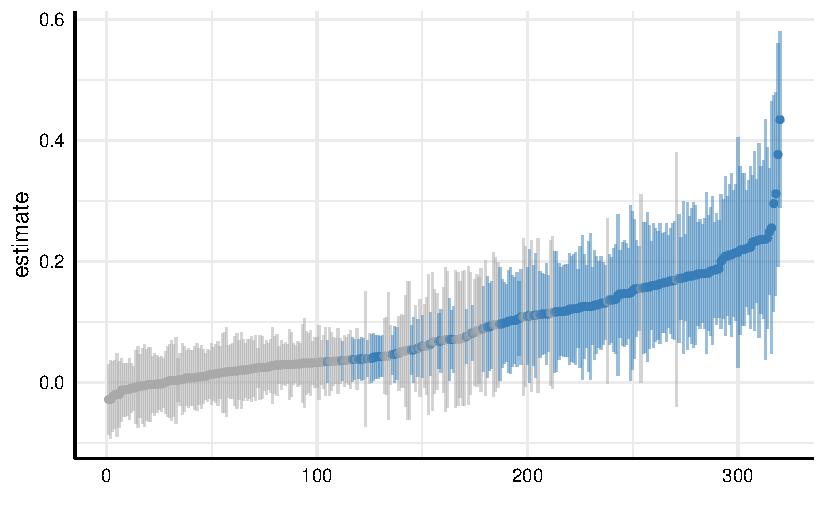
\includegraphics{PAPERLongTermImpactofWaronLifeSatisfaction_files/figure-pdf/results to show IIa-1.pdf}

Here again we find one factor that crucially affects conclusions: models
using the 1-5 life satisfaction scale produce much smaller and less
often significant effects, while most specifications using the 1-10 life
satisfaction scale find a positive and significant effect.

Figure IV: What Affects the Estimated Effect Size of Having Moved
Because of World War II on Life Satisfaction.

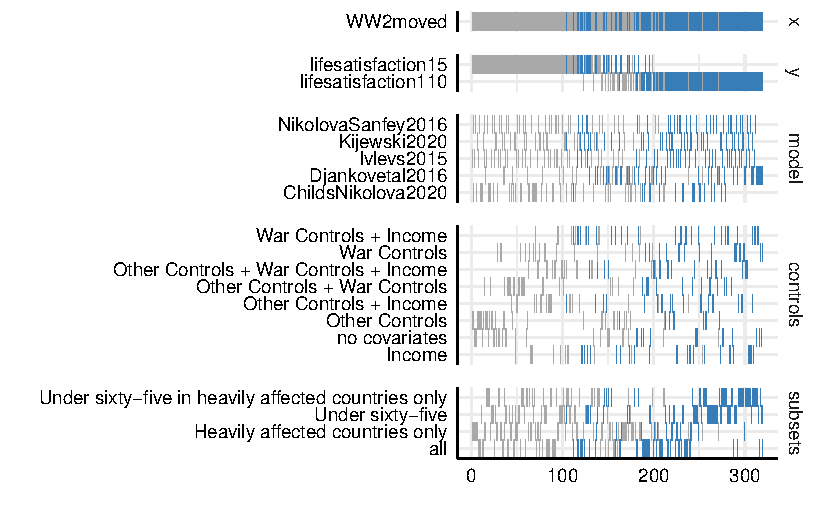
\includegraphics{PAPERLongTermImpactofWaronLifeSatisfaction_files/figure-pdf/results to show IIb-1.pdf}

Finally, we also explored the specification curves for the three recent
war variables: whether one was injured in a recent conflict, whether one
moved because of a recent conflict and whether one has family members
injured or killed because of a recent conflict. The effect size of these
variables varied a lot but few specifications showed significant
effects.

\hypertarget{v.-replicating-using-the-more-recent-lits-iii-data.}{%
\subsection{V. Replicating using the more recent LITS III
data.}\label{v.-replicating-using-the-more-recent-lits-iii-data.}}

So far, we worked with data from the second wave of the Life in
Transition Survey. In 2016, a third wave was implemented. In this
section, we analyse whether the conclusions of the original studies are
upheld when the more recent data are used.

The advantage of using the third wave is that the sample is bigger, with
about 1500 respondents per country being interviewed, compared to about
1000 in the second wave. While most control variables used by the
original studies are also available in the third wave, there are some
exceptions. Most importantly, only one life satisfaction question, the
one with the scale of 1 to 5, got asked in the third wave.

Table IV compares the results of the original studies with the
replicated results using the data from LITSIII. Interestingly, the
replication results with the new data are similar to the results
obtained by the original studies. Using Kijewski (2020) 's methodology,
we find a negative and significant effect, using Ivlevs (2015) 's
methodology, we find a positive and significant effect while the other
studies produce no significant effect. This suggest that if the original
authors had done their studies later, using LITSIII rather than LITSII,
they would have obtained similar conclusions in terms of the long-term
impact of war on life satisfaction.

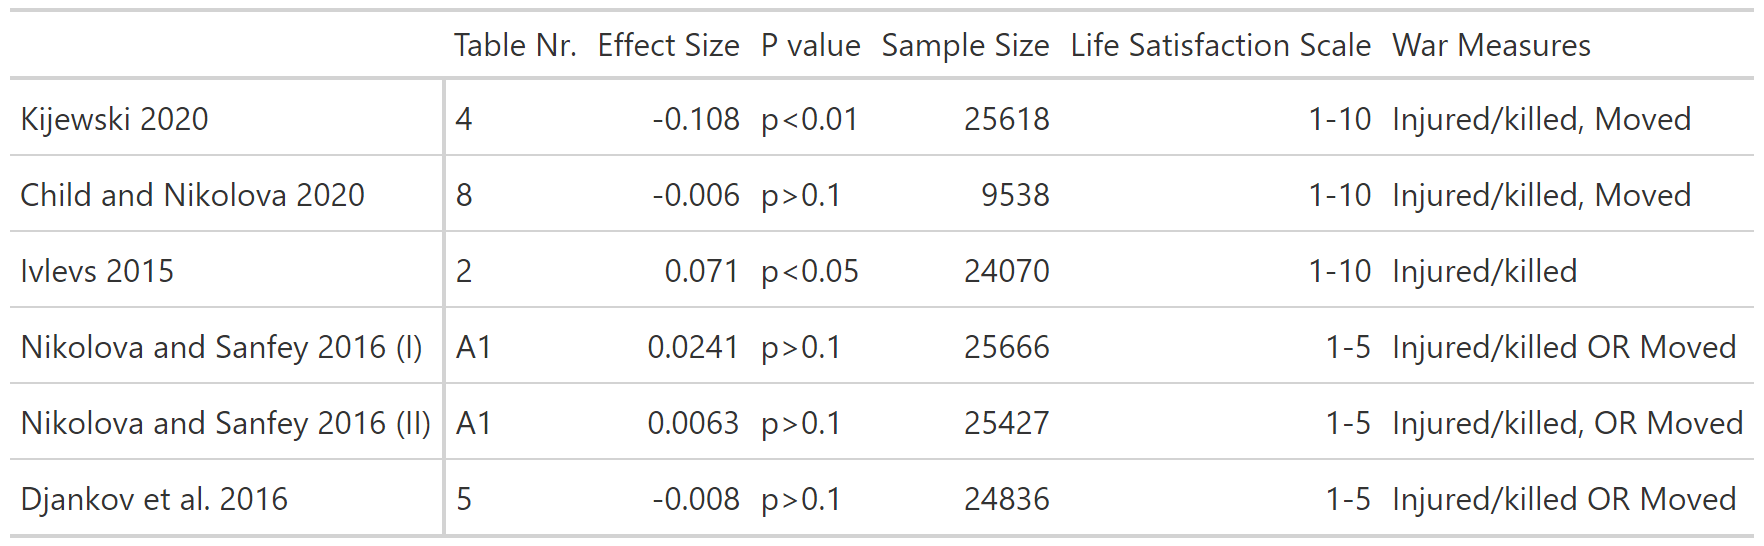
\includegraphics{tab_1.png}

\hypertarget{vi.-a-specification-curve-analysis-using-the-more-recent-data.}{%
\subsection{VI. A Specification Curve Analysis using the more recent
data.}\label{vi.-a-specification-curve-analysis-using-the-more-recent-data.}}

For completeness, our final step is to perform a specification curve
analysis with the more recent data from LITSIII.

As Figure V shows, we again find a wide range of results depending on
the specification choices we make. Interestingly, compared to Figure I
which mainly showed negative effects, using the third wave leads to many
more positive effects.

Figure V: A Specification Curve for the Impact of Being Injured/ Having
Injored or Killed Relatives during World War II on Life Satisfaction,
LITSIII.

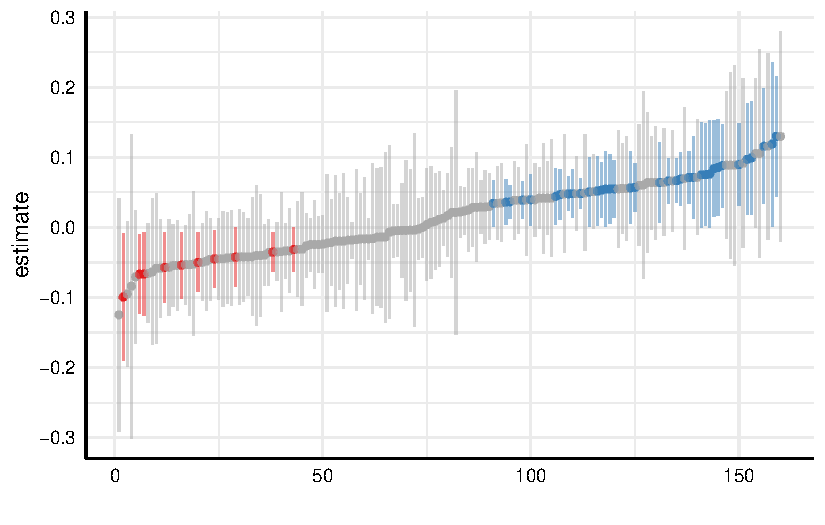
\includegraphics{PAPERLongTermImpactofWaronLifeSatisfaction_files/figure-pdf/results to show Ia iii-1.pdf}

Interestingly, the income variables are again crucially important for
the conclusions (see Figure VI). Like in Figure II including income
increases the estimated impact of the war variable. While in Figure I
this increase turned significantly negative estimates into insignificant
estimates, when using LITSIII, the increase one gets by including income
variables tends to push the estimated effect of the war variable from
insignificant to significantly positive.

Figure VI: What Affects the Estimated Effect Size of Being
Injured/Having Injured or Killed Relatives during World War II, LITSIII.

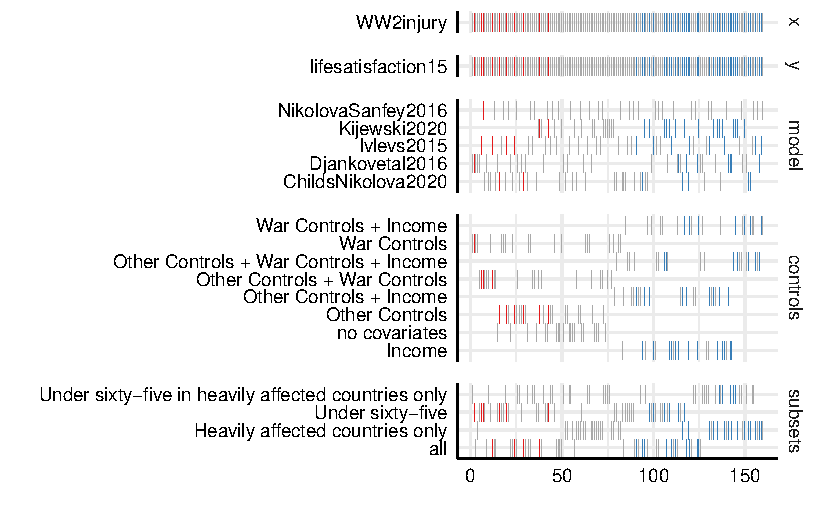
\includegraphics{PAPERLongTermImpactofWaronLifeSatisfaction_files/figure-pdf/results to show Ib iii-1.pdf}

\hypertarget{vii.-conclusions.}{%
\subsection{VII. Conclusions.}\label{vii.-conclusions.}}

In this paper, we replicate the literature that uses the second wave of
the Life in Transition Survey to estimate the impact of World War II on
life satisfaction, conduct a specification curve analysis, and update
the literature by also using data from the third wave of the survey.
While war experience is not fully randomized, limiting causal claims one
can make about its impact, the LITS II survey is a great source of
observational data to investigate the long-run relationship between war
and life satisfaction given it asks a large sample of respondents about
various war experiences, and measures life satisfactions in multiple
ways.

Given the suitability of the survey, it is no surprise that the
published literature using LITS II to regress life satisfaction on war
experience ( Kijewski (2020), Child and Nikolova (2020), Ivlevs (2015),
Nikolova and Sanfey (2016), Djankov, Nikolova, and Zilinsky (2016)) is
sizable. More surprising is that, depending on the paper one reads, one
can find a significant negative effect, a significant positive effect or
insignificant effects of World War II experience on life satisfaction,
despite these studies all using the same dataset and similar measures of
life satisfaction and war experience.

In this paper, we explore the reasons for this heterogeneity in
findings. Directly replicating the five papers using the LITS II data,
we find effect sizes and statistical significance that are similar to
those published. And even when using the more recent LITS III (2016
vs.~2010) to update these five papers we come to similar conclusions as
the original authors.

However, a specification curve analysis finds that, based on 320
`reasonable' specifications and the LITS II data, the impact of being
injured/having a family member being injured or killed during World War
II is mainly estimated to be negative but that these estimates are
statistically significant only when not including income as a control
variable. A specification curve analysis, based on 320 `reasonable'
specifications and the LITS III data, similarly shows the importance of
the including income variables but shows that the impact of being
injured/having a family member being injured or killed during World War
II is mainly estimated to be positive but that these estimates are
statistically significant only when including income as a control
variable.

We further show that the impact of having moved because of World War II
is mainly estimated to have a positive effect but only so when measuring
life satisfaction on a 1-10 scale (rather than a 1-5 scale). Finally, we
find little support for a significant effect of recent war experience on
life satisfaction.

Overall, this study shows that there is no easy answer to the question
whether experiencing a war has a long-term impact on life satisfaction.
The assumptions one chooses to make in terms of control variables,
measurement of life satisfaction and war experience, whether to weigh
observations or cluster standard errors, affect whether one obtains a
negative, positive, significant or insignificant estimate. Moreover, the
vast majority of specifications suggest the estimated impact is minor
when compared to the overall variation in life satisfaction. Hence,
using the Bradford-Hill criteria (Bradford-Hill (1965)), we would argue
that research about the long-term impact of war based on LITS data shows
low consistency and low strength, and thus provides little support for
there being a causal long-term effect of war experience on life
satisfaction.

This paper further adds to the literature that shows that the choices
researchers make when analysing a dataset can have a major impact on the
conclusions they draw. It is also a warning to readers that single
papers, even when including several robustness checks, do not
necessarily represent what one would learn from a comprehensive analysis
from the same dataset. The analysis here thus suggests a specification
curve analysis should be a part of any empirical paper, especially now
that software packages are available which make running hundreds of
specifications straightforward. Rather than focusing on robustness
checks that confirm the main finding of a paper, authors should focus on
revealing the true extent of model uncertainty.

\hypertarget{refs}{}
\begin{CSLReferences}{1}{0}
\leavevmode\vadjust pre{\hypertarget{ref-Adseraetal2021}{}}%
Adsera, Alıcia`and Francesca Dalla Pozza, Sergei Guriev, Lukas
Kleine-Rueschkamp, and Elena Nikolova. 2020. {``Height and Well-Being
During the Transition from Plan to Market.''} \emph{Economic Policy
January 2021, 77--120}.

\leavevmode\vadjust pre{\hypertarget{ref-Baker2016}{}}%
Baker, Monya. 2016. {``1,500 Scientists Lift the Lid on
Reproducibility.''} \emph{Nature, 533(7604), 452-454}.

\leavevmode\vadjust pre{\hypertarget{ref-BradfordHill1965}{}}%
Bradford-Hill, Austin. 1965. {``The Environment and Disease: Association
or Causation?''} \emph{Proceedings of the Royal Society of Medicine, 58
, 295-300}. \url{https://www.edwardtufte.com/tufte/hill}.

\leavevmode\vadjust pre{\hypertarget{ref-ChildNikolova2020}{}}%
Child, Travers Barclay, and Elena Nikolova. 2020. {``War and Social
Attitudes.''} \emph{Conflict Management and Peace Science, Vol. 37(2),
152--171}.
\url{https://journals.sagepub.com/doi/abs/10.1177/0738894217750564}.

\leavevmode\vadjust pre{\hypertarget{ref-CoupeObrizan2023}{}}%
Coupé, Tom, and Maksym Obrizan. 2023. {``War and Happiness.''}
\emph{Handbook of Subjective Well-Being}.

\leavevmode\vadjust pre{\hypertarget{ref-Djankovetal2016}{}}%
Djankov, Simeon, Elena Nikolova, and Jan Zilinsky. 2016. {``The
Happinessgap in Eastern Europe.''} \emph{Journal of Comparative
Economics, Vol. 44, 108--124}.
\url{https://www.sciencedirect.com/science/article/abs/pii/S0147596715000888}.

\leavevmode\vadjust pre{\hypertarget{ref-Hlavac2022}{}}%
Hlavac, Marek. 2022. {``Stargazer: Well-Formatted Regression and Summary
Statistics Tables. R Package Version 5.2.3.''}
\emph{Https://CRAN.R-Project.org/Package=stargazer}.

\leavevmode\vadjust pre{\hypertarget{ref-Hoogeveen2023}{}}%
Hoogeveen, Suzanne, Alexandra Sarafoglou, Balazs Aczel, Yonathan Aditya,
Alexandra J. Alayan, Peter J. Allen, Yulmaida Amir Sacha Altay Shilaan
Alzahawi, and Eric-Jan Wagenmakers. 2021. {``A Many-Analysts Approach to
the Relation Between Religiosity and Well-Being.''} \emph{Religion,
Brain \& Behavior, 13(3), 237-283}.

\leavevmode\vadjust pre{\hypertarget{ref-Huntington2021}{}}%
Huntington-Klein, Nicholas, Arenas A., Beam E., Bertoni M., J. Bloem,
Burli P., Chen N., et al. 2021. {``The Influence of Hidden Re-Searcher
Decisions in Applied Microeconomics.''} \emph{Economic Inquiry, 59(3),
944-960}.

\leavevmode\vadjust pre{\hypertarget{ref-Ivlevs2015}{}}%
Ivlevs, Artjoms. 2015. {``Happy Moves? Assessing the Link Between Life
Satisfaction and Emigration Intentions.''} \emph{Kyklos, Vol. 68(3),
335--356}.

\leavevmode\vadjust pre{\hypertarget{ref-Kijewski2020}{}}%
Kijewski, Sara. 2020. {``Life Satisfaction Sixty Years After World War
II: The Lasting Impact of War Across Generations.''} \emph{Applied
Research in Quality of Life, Vol. 15, 1253--1284}.
\url{https://link.springer.com/article/10.1007/s11482-019-09726-z}.

\leavevmode\vadjust pre{\hypertarget{ref-Masur2020}{}}%
Masur, Philipp K., and Michael Scharkow. 2020. {``Specr: Conducting and
Visualizing Specification Curve Analyses (Version 1.0.1).''}
\url{https://CRAN.R-project.org/package=specr}.

\leavevmode\vadjust pre{\hypertarget{ref-NikolovaSanfey2016}{}}%
Nikolova, Elena, and Peter Sanfey. 2016. {``How Much Should We Trust
Life Satisfaction Data? Evidence from the Life in Transition Survey.''}
\emph{Journal of Comparative Economics, Vol. 44, 720--731}.
\url{https://www.sciencedirect.com/science/article/abs/pii/S0147596715001122}.

\leavevmode\vadjust pre{\hypertarget{ref-Obrizan2019}{}}%
Obrizan, Maksym. 2019. {``Violent Conflict and Unhappiness: Evidence
from the 2016 `Life in Transition' III Survey.''} \emph{Economics
Bulletin, Vol.39(1), 192-199}.

\leavevmode\vadjust pre{\hypertarget{ref-Recher2022}{}}%
Recher, Vedran. 2022. {``History Matters: Life Satisfaction in
Transition Countries.''} \emph{Journal of Happiness Studies 23,
171--193}.

\leavevmode\vadjust pre{\hypertarget{ref-Reed2018}{}}%
Reed, W. Robert. 2018. {``A Primer on the {`Reproducibility Crisis'} and
Ways to Fix It.''} \emph{Australian Economic Review, 51(2), 286-300}.

\leavevmode\vadjust pre{\hypertarget{ref-Simonsohn2020}{}}%
Simonsohn, Uri, Simmons Joseph, and Leif Nelson. 2021. {``Specification
Curve Analysis.''} \emph{Nature Human Behavior 4, 1208--1214}.

\leavevmode\vadjust pre{\hypertarget{ref-Steegen2016}{}}%
Steegen, Sara, Francis Tuerlinckx, Andrew Gelman, and Wolf Vanpaemel.
2016. {``Increasing Transparency Through a Multiverse Analysis.''}
\emph{Perspectives on Psychological Science, 11(5) 702--712}.

\end{CSLReferences}



\end{document}
